\chapter{Reti sequenziali}
Fino ad ora abbiamo progettato circuiti combinatori con l'aiuto dell'algebra booleana. Con circuiti di questo tipo però viene esclusa la possibilità di creare cicli.
Vogliamo quindi passare ad altri tipi di circuiti, i cosidetti circuiti sequenziali, che ci permettono di memorizzare l'informazione attraverso linee di feedback.

\section{Latch SR}
Le prime che analizzeremo sono le latch SR, dove S e R stanno per set e reset.
La rappresentazione base di una latch SR è la seguente:

\begin{center}
    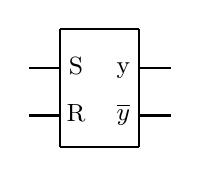
\begin{tikzpicture}
        % line
        \draw [thick] (0,0) -- (1,0);\draw [thick] (0,0) -- (0,1.5);\draw [thick] (0,1.5) -- (1,1.5);\draw [thick] (1,1.5) -- (1,0);
        
        \draw [thick] (0,0.4) -- (-0.4,0.4);\draw [thick] (0,1) -- (-0.4,1);
        \draw [thick] (1,0.4) -- (1.4,0.4);\draw [thick] (1,1) -- (1.4,1);
        % lecter
        \draw (0.2,0.2) -- (0.2,0.2) node [above] {\small{R}};\draw (0.2,0.8) -- (0.2,0.8) node [above] {\small{S}};\draw (0.8,0.75) -- (0.8,0.75) node [above] {\small{y}};\draw (0.8,0.15) -- (0.8,0.15) node [above] {\small{$\overline{y}$}};
    \end{tikzpicture}
\end{center}

\begin{center}
    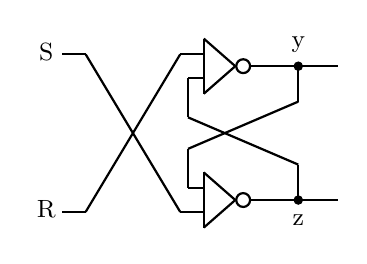
\begin{tikzpicture}
        % line
        \draw [thick] (0,0) -- (0.3,0);\draw [thick] (0,2) -- (0.3,2);
        \draw [thick] (0.3,0) -- (1.5,2);\draw [thick] (0.3,2) -- (1.5,0);
        \draw [thick] (1.5,2) -- (1.8,2);\draw [thick] (1.5,0) -- (1.8,0);
        
        \draw [thick] (2.4,0.15) -- (3.5,0.15);
        \draw [thick] (2.4,1.85) -- (3.5,1.85);
        \draw [thick] (3,0.15) -- (3,0.6);\draw [thick] (3,1.85) -- (3,1.4);
        \draw [thick] (3,1.4) -- (1.6,0.8);\draw [thick] (3,0.6) -- (1.6,1.2);
        
        \draw [thick] (1.6,0.8) -- (1.6,0.3);\draw [thick] (1.6,0.3) -- (1.8,0.3);
        \draw [thick] (1.6,1.2) -- (1.6,1.7);\draw [thick] (1.6,1.7) -- (1.8,1.7);
        % triangle and point
        \draw [thick] (1.8,-0.2) -- (1.8,0.5);\draw [thick] (1.8,0.5) -- (2.2,0.15);\draw [thick] (1.8,-0.2) -- (2.2,0.15);\draw[thick, black] (2.3,0.15) circle (2.5pt);
        \draw [thick] (1.8,2.2) -- (1.8,1.5);\draw [thick] (1.8,1.5) -- (2.2,1.85);
        \draw [thick] (1.8,2.2) -- (2.2,1.85);\draw[thick, black] (2.3,1.85) circle (2.5pt);
        
        % lecter
        \draw (-0.2,-0.2) -- (-0.2,-0.2) node [above] {\small{R}};\draw (-0.2,1.8) -- (-0.2,1.8) node [above] {\small{S}};
        \draw (3,1.9) -- (3,1.9) node [above] {\small{y}};\draw (3,-0.3) -- (3,-0.3) node [above] {\small{z}};
        % point
        \filldraw[black] (3,1.85) circle (1.5pt);\filldraw[black] (3,0.15) circle (1.5pt);
    \end{tikzpicture}
\end{center}

y rappresenta lo stato del latch e il valore del bit memorizzato. Dando dei valori binari ad S e R posso memorizzare o cambiare il valore di y:

\begin{enumerate}
    \item Per \textbf{memorizzare} un valore, devo impostare S e R a 0.
    
    Per capire perchè ciò avviene, "tagliamo" la seconda uscita di y e le estremità le identifichiamo come A e B.
    L'espressione di y diventa:
    \begin{equation*}
        y=\overline{R+\overline{S+A}}=\overline{R}(S+A)
    \end{equation*}
    Ora se poniamo A = 1 otteniamo $y=1(0+1)=1$. Essendo A = B notiamo come abbiamo ottenuto lo stesso risultato.
    
    Se poniamo A = 0 otteniamo $y=(0+0)=0$. Anche in questo caso A = B quindi possiamo ricongiungere la linea spezzata.
    
    Notiamo come con R e S = 0 il valore si mantiene possiamo quindi scrivere la nostra funzione di memorizzazione come:
    \begin{equation}\label{eq:ylatchSR}
        y=\overline{R+z}=\overline{R+\overline{(S+y)}}=\overline{R}(S+y)
    \end{equation}
    Può sembrare strano che per calcolare y sto usando ancora una volta y ma dobbiamo tener presente che sono due valori diversi perchè osservati in tempi diversi. Per chiarezza la prima y viene chiamata y(t+1) mentre la seconda (ricavata da z) y(t). t+1 è il tempo che mi serve per attraversare le porte NOR.
    
    \item Per \textbf{impostare} un valore, devo ottenere y = 1 nello stato del latch.
    \begin{enumerate}
        \item Se S = 1 e R = 0 stiamo generando una funzione di \textbf{set}:
        
        Per y = 0 abbiamo che $z=\overline{S+y}=\overline{1+0}=0$ quindi $y=\overline{R+z}=\overline{0+0}=1$.
        
        Per y = 1 abbiamo che $z=\overline{S+y}=\overline{1+1}=0$ quindi $y=\overline{R+z}=\overline{0+0}=1$.
        
        Notiamo come in entrambe i casi il valore della y è stato impostato a 1 (anche se nel secondo caso non è visibile).
        
        \item Con S = 0 e R = 1 generiamo una funzione di \textbf{reset}:
        
        Per y = 1 e z = 0 abbiamo che $y=\overline{R+z}=\overline{1+0}=0$ e $z=\overline{S+y}=\overline{0+0}=1$.
        
        Per y = 0 e z = 1 abbiamo che $y=\overline{R+z}=\overline{1+1}=0$ e $z=\overline{S+y}=\overline{0+0}=1$.
        
        In entrambe i casi la y è stata impostata a valore 0.
    \end{enumerate}
    
    \item Otteniamo una configurazione non ammessa quando sia S che R valgono 1 e la nostra relazione perde così di significato. 
    Questo perchè con y e z = 0 si perde la relazione fondamentale $z=\overline{y}$.
\end{enumerate}

\begin{table}[ht]
    \centering
    \begin{tabular}{|c|c|c|}
         \hline SR & y(t+1) & Func.\\\hline\hline
         00 & y(t) & Memorizzazione\\\hline
         01 & 0 & Reset\\\hline
         10 & 1 & Set\\\hline
         11 & - & Non ammessa\\\hline
    \end{tabular}
    \caption{Tabella del latch SR}
    \label{tab:latch_SR}
\end{table}

Come abbiamo visto quando il segnale passa attraverso delle porte si ha un piccolo ritardo chiamato $\Delta (t)$. Per tanto, nei computer, si utilizza un segnale chiamato clock che ha una sua frequenza e un suo periodo.

Le latch sono reti sensibili alla temporizzazione. Quando aggiungiamo un latch con un orologio otteniamo un gated latch o \textbf{flip-flop}.

\begin{center}
    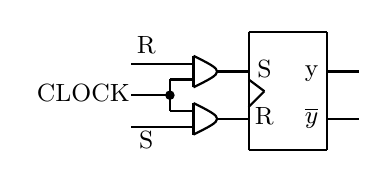
\begin{tikzpicture}
        % line
        \draw [thick] (0,0) -- (1,0);\draw [thick] (0,0) -- (0,1.5);\draw [thick] (0,1.5) -- (1,1.5);\draw [thick] (1,1.5) -- (1,0);
        
        \draw [thick] (0,0.4) -- (-0.4,0.4);\draw [thick] (0,1) -- (-0.4,1);
        \draw [thick] (1,0.4) -- (1.4,0.4);\draw [thick] (1,1) -- (1.4,1);
        
        \draw [thick] (-0.7,0.5) -- (-1,0.5);\draw [thick] (-0.7,0.3) -- (-1.5,0.3);
        \draw [thick] (-1,0.5) -- (-1,0.9);\filldraw[black] (-1,0.7) circle (1.5pt);\draw [thick] (-1,0.7) -- (-1.5,0.7);
        \draw [thick] (-0.7,0.9) -- (-1,0.9);\draw [thick] (-0.7,1.1) -- (-1.5,1.1);
        % lecter
        \draw (0.2,0.2) -- (0.2,0.2) node [above] {\small{R}};\draw (0.2,0.8) -- (0.2,0.8) node [above] {\small{S}};\draw (0.8,0.75) -- (0.8,0.75) node [above] {\small{y}};\draw (0.8,0.15) -- (0.8,0.15) node [above] {\small{$\overline{y}$}};
        
        \draw (-1.3,1.1) -- (-1.3,1.1) node [above] {\small{R}};\draw (-1.3,-0.1) -- (-1.3,-0.1) node [above] {\small{S}};\draw (-2.1,0.5) -- (-2.1,0.5) node [above] {\small{CLOCK}};
        % curve
        \draw [thick] (-0.7,0.2) -- (-0.7,0.6);\draw[thick] (-0.7,0.2) .. controls (-0.3,0.4) .. (-0.7,0.6);
        \draw [thick] (-0.7,0.8) -- (-0.7,1.2);\draw[thick] (-0.7,0.8) .. controls (-0.3,1) .. (-0.7,1.2);
        % tringle
        \draw [thick] (0.2,0.75) -- (0,0.55);\draw [thick] (0.2,0.75) -- (0,0.9);
    \end{tikzpicture}
\end{center}

\begin{center}
    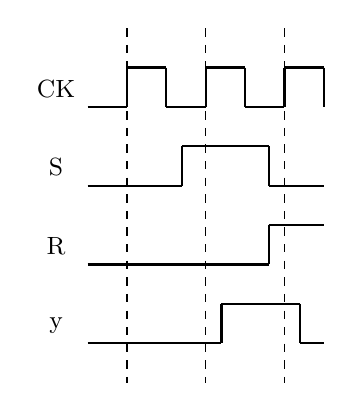
\begin{tikzpicture}
        % line
        \draw [thick] (0,0) -- (0.5,0);\draw [thick] (0.5,0) -- (0.5,0.5);\draw [thick] (0.5,0.5) -- (1,0.5);\draw [thick] (1,0.5) -- (1,0);\draw [thick] (1,0) -- (1.5,0);\draw [thick] (1.5,0) -- (1.5,0.5);\draw [thick] (1.5,0.5) -- (2,0.5);\draw [thick] (2,0.5) -- (2,0);\draw [thick] (2,0) -- (2.5,0);\draw [thick] (2.5,0) -- (2.5,0.5);\draw [thick] (2.5,0.5) -- (3,0.5);\draw [thick] (3,0.5) -- (3,0);
        \draw [thick] (0,-1) -- (1.2,-1);\draw [thick] (1.2,-1) -- (1.2,-0.5);\draw [thick] (1.2,-0.5) -- (2.3,-0.5);\draw [thick] (2.3,-0.5) -- (2.3,-1);\draw [thick] (2.3,-1) -- (3,-1);
        \draw [thick] (0,-3) -- (1.7,-3);\draw [thick] (1.7,-3) -- (1.7,-2.5);\draw [thick] (1.7,-2.5) -- (2.7,-2.5);\draw [thick] (2.7,-2.5) -- (2.7,-3);\draw [thick] (2.7,-3) -- (3,-3);
        \draw [thick] (0,-2) -- (2.3,-2);\draw [thick] (2.3,-2) -- (2.3,-1.5);\draw [thick] (2.3,-1.5) -- (3,-1.5);
        % lecter
        \draw (-0.4,0) -- (-0.4,0) node [above] {\small{CK}};
        \draw (-0.4,-1) -- (-0.4,-1) node [above] {\small{S}};
        \draw (-0.4,-2) -- (-0.4,-2) node [above] {\small{R}};
        \draw (-0.4,-3) -- (-0.4,-3) node [above] {\small{y}};
        % pointed
        \draw [dashed] (0.5,1) -- (0.5,-3.5);
        \draw [dashed] (1.5,1) -- (1.5,-3.5);
        \draw [dashed] (2.5,1) -- (2.5,-3.5);
    \end{tikzpicture}
\end{center}
Questo accade perchè il cambiamento di S ed R viene catturato sul fronte di salita del clock e successivamente y, con un ritardo $\Delta(t)$, viene impostato al valore corretto.

\section{Flip-flop D}
Il flip-flop di delay deriva dal latch SR e si chiama così perchè il valore di ingresso viene riportato con un certo delay in uscita.

\begin{center}
    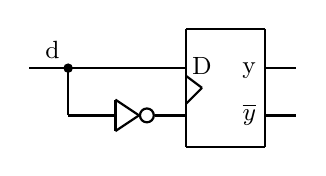
\begin{tikzpicture}
        % line
        \draw [thick] (0,0) -- (1,0);\draw [thick] (0,0) -- (0,1.5);\draw [thick] (0,1.5) -- (1,1.5);\draw [thick] (1,1.5) -- (1,0);
        \draw [thick] (1,0.4) -- (1.4,0.4);\draw [thick] (1,1) -- (1.4,1);
        
        \draw [thick] (0,0.4) -- (-0.4,0.4);\draw [thick] (0,1) -- (-0.4,1);
        \draw [thick] (-0.4,1) -- (-2,1);\draw [thick] (-1.5,1) -- (-1.5,0.4);\draw [thick] (-1.5,0.4) -- (-0.9,0.4);
        % lecter
        \draw (0.2,0.8) -- (0.2,0.8) node [above] {\small{D}};\draw (0.8,0.75) -- (0.8,0.75) node [above] {\small{y}};\draw (0.8,0.15) -- (0.8,0.15) node [above] {\small{$\overline{y}$}};
        \draw (-1.7,1) -- (-1.7,1) node [above] {\small{d}};
        % triangle and point
        \draw [thick] (0.2,0.75) -- (0,0.55);\draw [thick] (0.2,0.75) -- (0,0.9);
        \draw [thick] (-0.9,0.2) -- (-0.9,0.6);\draw [thick] (-0.9,0.2) -- (-0.6,0.4);\draw [thick] (-0.6,0.4) -- (-0.9,0.6);\draw[thick, black] (-0.5,0.4) circle (2.5pt);
        \filldraw[black] (-1.5,1) circle (1.5pt);
    \end{tikzpicture}
\end{center}

\begin{table}[ht]
    \centering
    \begin{tabular}{c|c}
         d & y(t+1)\\\hline
         0 & 0\\
         1 & 1
    \end{tabular}
\end{table}

In un flip-flop di delay si assume come ingresso solo una variabile $d$ vera e complementata. Con una configurazione del genere, gli ingressi non possono mai essere 0 0 o 1 1, ma si otterranno solo funzioni set o reset.

\section{Flip-flop JK}
Il flip-flop JK deriva del latch SR.
\begin{center}
    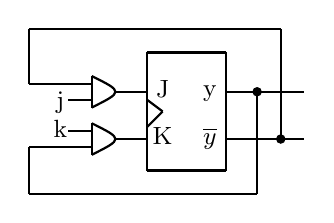
\begin{tikzpicture}
        % line
        \draw [thick] (0,0) -- (1,0);\draw [thick] (0,0) -- (0,1.5);\draw [thick] (0,1.5) -- (1,1.5);\draw [thick] (1,1.5) -- (1,0);
        
        \draw [thick] (0,0.4) -- (-0.4,0.4);\draw [thick] (0,1) -- (-0.4,1);
        \draw [thick] (1,0.4) -- (2,0.4);\draw [thick] (1,1) -- (2,1);
        
        \draw [thick] (-0.7,0.5) -- (-1,0.5);\draw [thick] (-0.7,0.3) -- (-1.5,0.3);
        \draw [thick] (-0.7,0.9) -- (-1,0.9);\draw [thick] (-0.7,1.1) -- (-1.5,1.1);
        
        \draw [thick] (-1.5,0.3) -- (-1.5,-0.3);\draw [thick] (-1.5,-0.3) -- (1.4,-0.3);\draw [thick] (1.4,-0.3) -- (1.4,1);
        \draw [thick] (-1.5,1.1) -- (-1.5,1.8);\draw [thick] (-1.5,1.8) -- (1.7,1.8);\draw [thick] (1.7,1.8) -- (1.7,0.4);
        % lecter
        \draw (0.2,0.2) -- (0.2,0.2) node [above] {\small{K}};\draw (0.2,0.8) -- (0.2,0.8) node [above] {\small{J}};\draw (0.8,0.75) -- (0.8,0.75) node [above] {\small{y}};\draw (0.8,0.15) -- (0.8,0.15) node [above] {\small{$\overline{y}$}};
        \draw (-1.1,0.6) -- (-1.1,0.6) node [above] {\small{j}};
        \draw (-1.1,0.3) -- (-1.1,0.3) node [above] {\small{k}};
        % point
        \filldraw[black] (1.7,0.4) circle (1.5pt);\filldraw[black] (1.4,1) circle (1.5pt);
        % curve
        \draw [thick] (-0.7,0.2) -- (-0.7,0.6);\draw[thick] (-0.7,0.2) .. controls (-0.3,0.4) .. (-0.7,0.6);
        \draw [thick] (-0.7,0.8) -- (-0.7,1.2);\draw[thick] (-0.7,0.8) .. controls (-0.3,1) .. (-0.7,1.2);
        % triangle
        \draw [thick] (0.2,0.75) -- (0,0.55);\draw [thick] (0.2,0.75) -- (0,0.9);
    \end{tikzpicture}
\end{center}

Ricordando l'Equazione \ref{eq:ylatchSR} avevamo che $y(t+1)=\overline{R}(S+y)$, ma in questa configurazione abbiamo $S=j\overline{y}$ e $R=yk$.
Sostituiendoli nella y otteniamo: $y(t+1)=(j\overline{y}+y)\overline{yk}$ = De Morgan = $y(t+1)=(j\overline{y}+y)(\overline{y}+\overline{k})$ = assorbimento = $y(t+1)=(j+y)(\overline{y}+\overline{k})$ = svolgendo i prodotti ottengo = $y(t+1)=j\overline{y}+j\overline{k}+y\overline{y}+y\overline{k}$ =
\begin{equation*}
    y(y+1)=j\overline{y}+j\overline{k}+y\overline{k}
\end{equation*}

A questo punto avremo che se:
\begin{itemize}
    \item j = 0 e k = 0 $\hspace{0,5cm}y(t+1)=y$
    \item j = 0 e k = 1 $\hspace{0,5cm}y(t+1)=0$
    \item j = 1 e k = 0 $\hspace{0,5cm}y(t+1)=\overline{y}+1+y=1$
    \item j = 1 e k = 1 $\hspace{0,5cm}y(t+1)=\overline{y}$
\end{itemize}

\begin{table}[ht]
    \centering
    \begin{tabular}{|c|c|c|}
         \hline jk & y(t+1) & Func.\\\hline\hline
         00 & y(t) & Memorizzazione\\\hline
         01 & 0 & Reset\\\hline
         10 & 1 & Set\\\hline
         11 & $\overline{y(t)}$ & Complemento\\\hline
    \end{tabular}
    \caption{Tabella del flip-flop JK}
\end{table}

\section{Flip-flop T}
Il flip-flop T (toggle) deriva dal latch SR.

\begin{center}
    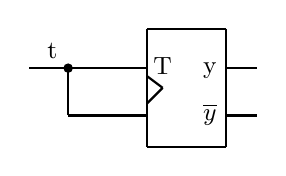
\begin{tikzpicture}
        % line
        \draw [thick] (0,0) -- (1,0);\draw [thick] (0,0) -- (0,1.5);\draw [thick] (0,1.5) -- (1,1.5);\draw [thick] (1,1.5) -- (1,0);
        \draw [thick] (1,0.4) -- (1.4,0.4);\draw [thick] (1,1) -- (1.4,1);
        
        \draw [thick] (0,0.4) -- (-0.4,0.4);\draw [thick] (0,1) -- (-0.4,1);
        \draw [thick] (-0.4,1) -- (-1.5,1);\draw [thick] (-1,1) -- (-1,0.4);\draw [thick] (-0.4,0.4) -- (-1,0.4);
        
        % lecter
        \draw (0.2,0.8) -- (0.2,0.8) node [above] {\small{T}};\draw (0.8,0.75) -- (0.8,0.75) node [above] {\small{y}};\draw (0.8,0.15) -- (0.8,0.15) node [above] {\small{$\overline{y}$}};
        \draw (-1.2,1) -- (-1.2,1) node [above] {\small{t}};
        % triangle and point
        \draw [thick] (0.2,0.75) -- (0,0.55);\draw [thick] (0.2,0.75) -- (0,0.9);
        \filldraw[black] (-1,1) circle (1.5pt);
    \end{tikzpicture}
\end{center}

Questo tipo di configurazione può assumere solo i valori j = 0 e k = 0 o j = 1 e k = 1.
\begin{table}[ht]
    \centering
    \begin{tabular}{c|c}
         t & y(t+1)\\\hline
         0 & y(t+1)\\
         1 & $\overline{y(t+1)}$
    \end{tabular}
\end{table}

\section{Analisi e sintesi di una rete sequenziale}
\begin{center}
    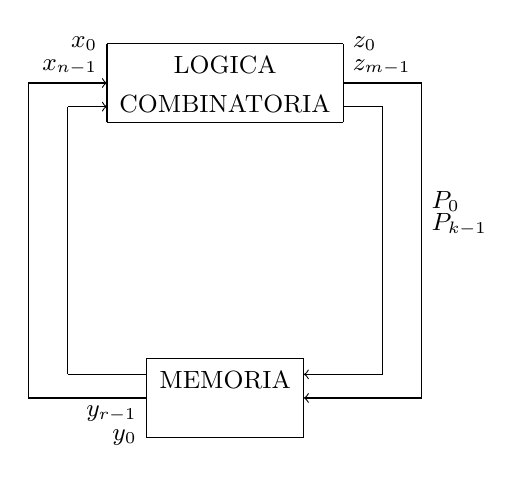
\begin{tikzpicture}
        % line
        \draw (0,0) -- (2,0);\draw (2,0) -- (2,1);\draw (0,0) -- (0,1);\draw (0,1) -- (2,1);
        \draw (-0.5,4) -- (2.5,4);\draw (2.5,4) -- (2.5,5);\draw (-0.5,4) -- (-0.5,5);\draw (-0.5,5) -- (2.5,5);
        
        \draw (0,0.8) -- (-1,0.8);\draw (-1,0.8) -- (-1,4.2);\draw[->] (-1,4.2) -- (-0.5,4.2);
        \draw (0,0.5) -- (-1.5,0.5);\draw (-1.5,0.5) -- (-1.5,4.5);\draw[->] (-1.5,4.5) -- (-0.5,4.5);
        
        \draw[<-] (2,0.8) -- (3,0.8);\draw (3,0.8) -- (3,4.2);\draw (3,4.2) -- (2.5,4.2);
        \draw[<-] (2,0.5) -- (3.5,0.5);\draw (3.5,0.5) -- (3.5,4.5);\draw (3.5,4.5) -- (2.5,4.5);
        
        % lecter
        \draw (1,0.5) -- (1,0.5) node [above] {\small{MEMORIA}};
        \draw (1,4.5) -- (1,4.5) node [above] {\small{LOGICA}};
        \draw (1,4) -- (1,4) node [above] {\small{COMBINATORIA}};
        \draw (0,0) -- (0,0) node [left] {\small{$y_0$}};
        \draw (0,0.3) -- (0,0.3) node [left] {\small{$y_{r-1}$}};
        \draw (-0.5,5) -- (-0.5,5) node [left] {\small{$x_0$}};
        \draw (-0.5,4.7) -- (-0.5,4.7) node [left] {\small{$x_{n-1}$}};
        \draw (2.5,5) -- (2.5,5) node [right] {\small{$z_0$}};
        \draw (2.5,4.7) -- (2.5,4.7) node [right] {\small{$z_{m-1}$}};
        \draw (3.5,3) -- (3.5,3) node [right] {\small{$P_0$}};
        \draw (3.5,2.7) -- (3.5,2.7) node [right] {\small{$P_{k-1}$}};
    \end{tikzpicture}
\end{center}
$x_0\text{ e }x_{x-1}$ sono gli ingressi, $z_0\text{ e }z_{m-1}$ sono le uscite, $P_0\text{ e }P_{k-1}$ sono le funzioni di eccitazione.

Le reti sequenziali sono reti più sofisticate dove, oltre alla parte combinatoria, abbiamo anche quella di memoria.
Possiamo distinguere, anche per le reti sequenzali, i processi di analisi e sintesi:
\begin{enumerate}
    \item[a)] \textbf{Analisi:} Data una rete usiamo un procedimento per interpretare cosa produce.
    \item[b)] \textbf{Sintesi:} Data la specifica verbale usiamo un procedimento per progettare la rete minima.
\end{enumerate}

\subsection*{Analisi}
Il procedimento per l'analisi di una rete sequenziale è il seguente:
\begin{enumerate}
    \item\label{rs_ana_1} Produrre le espressioni booleane delle uscite;
    \item\label{rs_ana_2} Produrre le espressioni booleane delle funzioni di eccitazione;
    \item\label{rs_ana_3} Impostare la tavola degli stati futuri;
    \item\label{rs_ana_4} Construire il diagramma di stato (automa a stati finiti o macchina a stati finiti);
    \item\label{rs_ana_5} Scrivere la descrizione verbale.
\end{enumerate}

Utilizziamo ora il seguente esempio per capire meglio l'analisi di una rete sequenziale:
\begin{example}
    \begin{figure}[ht]
        \centering
        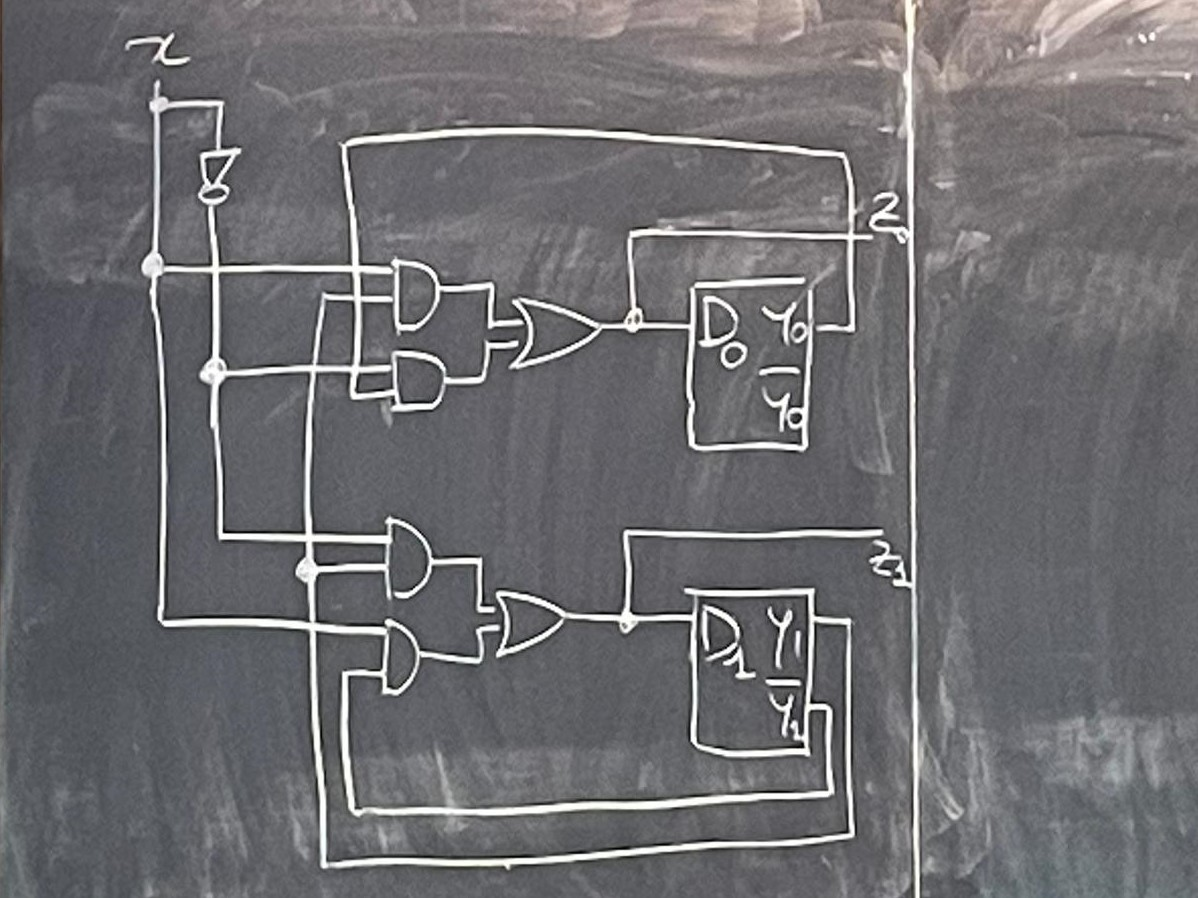
\includegraphics[width = 8cm]{images/reti_seq_es.jpeg}
        \caption{Rete sequenziale con Flip-flop di delay}
        \label{fig:es:reti_seq}
    \end{figure}
    
    \ref{rs_ana_1}, \ref{rs_ana_2} Scriviamo le espressioni booleane delle uscite e delle funzioni di eccitazione (che in questo caso coincidono).
    \begin{equation*}
        z_0=xy_1+\overline{x}y_0=D_0\hspace{0,5cm}
        z_1=\overline{x}y_1+x\overline{y_1}=D_1
    \end{equation*}
    
    \ref{rs_ana_3} La tavola degli stati futuri, serve per capire quali saranno i risultati della nostra funzione. E' un modo di rappresentare i dati che abbiamo molto utile perchè ci mostra tutto ciò che può accadere in tutti i casi.
    
    La tavola di compone di quattro colonne. Nella prima troveremo gli ingressi e gli stati rappresentati come combinazioni di valori binari. Nella seconda e terza colonna ci sono rispettivamente le funzioni di eccitazione e di uscita. Nell'ultima colonna rappresentiamo gli stati futuri.
    
    Guardando le espressioni booleane sopra scritte ci chiediamo per quali valori di $y_1$ e $y_0$ le funzioni di eccitazione valgono 1? E per quelle di uscita?
    
    \begin{table}[ht]
        \centering
        \begin{tabular}{|c|c|c|c|}
             \hline $xy_1y_0$ & $D_1D_0$ & $z_1z_0$ & $y_1y_0$\\\hline\hline
             000 & 00 & 00 & 00\\
             001 & 01 & 01 & 01\\
             010 & 10 & 10 & 10\\
             011 & 10 & 11 & 11\\\hline
             100 & 10 & 10 & 10\\
             101 & 10 & 10 & 10\\
             110 & 01 & 01 & 01\\
             111 & 01 & 01 & 01\\\hline
        \end{tabular}
        \caption{Tavola degli stati futuri}
    \end{table}
    
    Infine avremo tanti stati futuri quanti sono i flip-flop nella rete.
    I valori degli stati futuri in questo caso sono uguali a quelli degli stati di eccitazione perchè nel flip-flop di delay quando $d=0$, $y(t+1)=0$ e quando $d=1$, $y(t+1)=1$.
    
    \ref{rs_ana_4} Volendo rappresentare in forma grafica la tabella possiamo costruire quello che viene chiamato il diagramma di stato o automa.
    
    Per rappresentarlo dobbiamo scrivere tutti gli stati (tutte le possibili combinazioni di memoria), raffigurati da cerchi etichettati con la configurazione di memoria.
    
    Rappresentiamo poi la transizione tra uno stato e l'altro (passaggio da stato attuale a stato futuro a fronte dei valori di ingresso) tramite delle frecce etichettate da valore di ingresso/valore di uscita.
    
    Seguendo i passaggi il risultato sarà il seguente:
    \begin{figure}[ht]
        \centering
        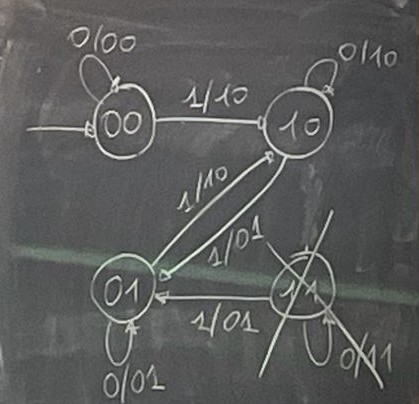
\includegraphics[width = 6cm]{images/reti_seq_automa_es.jpeg}
        \caption{Automa a stati finiti}
    \end{figure}
    
    Possiamo infine identificare uno stato di ingresso o eliminare gli eventuali stati che non verranno mai raggiunti.
    
    Per generalizzare il funzionamento della rete, possiamo assegnare dei nomi simbolici agli stati e agli ingressi, in modo da rendere più semplice il processo di descrizione della rete.
\end{example}

\subsection*{Sintesi}
Per sviluppare un buon processo di sintesi possiamo seguire questi passi:
\begin{itemize}
    \item Descrizione varbale;
    \item Automa della macchina a stati finiti (vedi Sezione \ref{sec:automa_asf});
    \item Automa della rete sequenziale (tramite l'assegnamento della codifica binaria a stati, ingressi e uscite);
    \item Tavola degli stati futuri (vedi Sezione \ref{sec:tabinvff});
    \item Espressioni booleane delle funzioni di eccitazione e delle uscite;
    \item Disegno della rete sequenziale.
\end{itemize}

Per un'esempio completo, vedi Esercizio \ref{es:sintesi_retseq}.

\subsubsection*{Tabelle inverse dei flip-flop}\label{sec:tabinvff}
Per progettare la nostra rete dobbiamo capire quando valgono le funzioni di eccitazione.

Per qualisiasi tipo di flip-flop che consideriamo, il procedimento si svolge sempre allo stesso modo: mi chiedo \textit{passando da y a Y quale funzione o valore ottengo nel flip-flop considerato?}

Ad esempio nel flip-flop SR, passando da 0 a 0 produco le fuzioni di memorizzazione e di reset. Produco infatti 0 e $\delta$, in quanto 00 vale per la funzione di memorizzazine e 01 per quella di reset. Si procede in questo modo completando la tabella inversa:
\begin{itemize}
    \item Flip-flop SR
    \begin{tabular}{c|c}
         $yY$&$SR$\\\hline
         00&0$\delta$\\
         01&10\\
         10&01\\
         11&$\delta$0
    \end{tabular}
    \item Flip-flop D
    \begin{tabular}{c|c}
         $yY$&$d$\\\hline
         00&0\\
         01&1\\
         10&0\\
         11&1
    \end{tabular}
    \item Flip-flop JK
    \begin{tabular}{c|c}
         $yY$&$jk$\\\hline
         00&0$\delta$\\
         01&1$\delta$\\
         10&$\delta$1\\
         11&$\delta$0
    \end{tabular}
    \item Flip-flop T
    \begin{tabular}{c|c}
         $yY$&$t$\\\hline
         00&0\\
         01&1\\
         10&1\\
         11&0
    \end{tabular}
    
\end{itemize}


\subsubsection*{Automa a stati finiti}\label{sec:automa_asf}
Un'automa a stati finiti (o Finitate State Automata/Machine) rappresenta un'automa con un numero finito di stati.
Per descriverlo utilizziamo un'insieme di oggetti:

\begin{table}[ht]
    \centering
    \begin{tabular}{|cc|}
         \hline Descrizione & Simbolo\\\hline
         Insieme finito di stati & $Q$\\
         Insieme finito di ingressi & $\varepsilon$\\
         Funzione di transizione & $\delta$\\
         Stato iniziale & $q_0$\\
         Valori di uscita & $U$\\
         Funzione di uscita & $\lambda$\\\hline
    \end{tabular}
    \caption{Oggetti dell'automa}
    \label{tab:autom_ogg}
\end{table}

Tra gli oggetti rappresentati in Tabella \ref{tab:autom_ogg}, abbiamo due funzioni. La prima (funzione di transizione) ci permette di stabilire lo stato futuro nella rappresentazione, dove nel grafico viene espressa tramite una freccia. Essendo una funzione possiamo identificare dominio e codominio:
\begin{equation*}
    \delta:Qx\varepsilon\rightarrow Q
\end{equation*}
La seconda (funzione di uscita) viene rappresentata tramite l'automa di Mealy o tramite l'automa di Moore a cui fanno riferimento, rispettivamente, le seguenti due funzioni:
\begin{equation*}
    \lambda:Qx\varepsilon\rightarrow U\hspace{1cm}\lambda:Q\rightarrow U
\end{equation*}

Facciamo un'esempio per capire meglio le differenze tra le due rappresentazioni.

\begin{example}
Ipotizziamo di avere la seguente tabella dell'automa:

    \begin{table}[ht]
        \centering
        \begin{tabular}{|c|c|c|}
             \hline& a & b\\\hline
             $S_0$& \diagbox[width=1cm]{$S_1$}{A} & \diagbox[width=1cm]{$S_2$}{B}\\\hline
             $S_1$&\diagbox[width=1cm]{$S_0$}{A} & \diagbox[width=1cm]{$S_3$}{B}\\\hline
             $S_2$&\diagbox[width=1cm]{$S_1$}{B} & \diagbox[width=1cm]{$S_3$}{A}\\\hline
             $S_3$&\diagbox[width=1cm]{$S_2$}{B} & \diagbox[width=1cm]{$S_1$}{B}\\\hline
        \end{tabular}
    \end{table}
    
    \begin{figure}[ht]
        \centering
        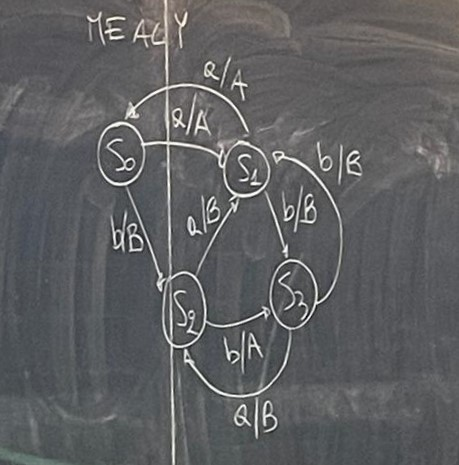
\includegraphics[height = 6cm]{images/mealy.jpeg}\hspace{0.5cm}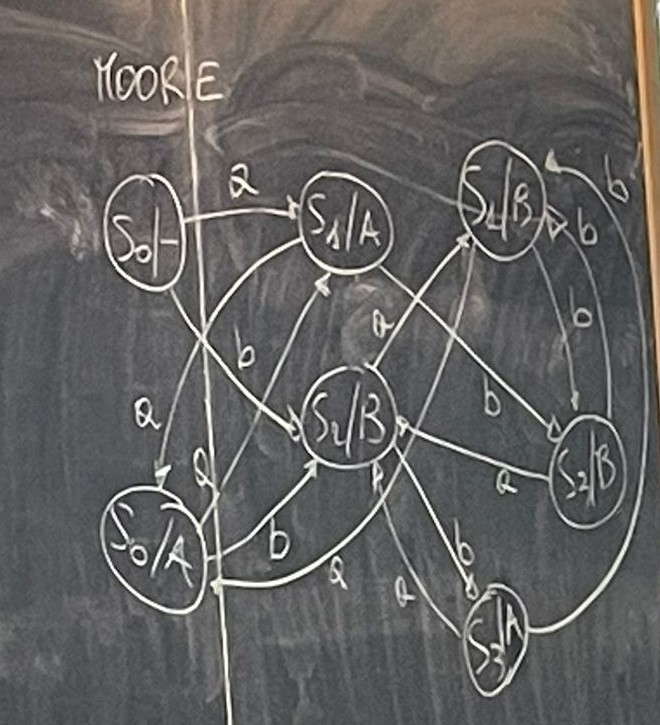
\includegraphics[height = 6cm]{images/moore.jpeg}
        \caption{Automa di Mealy e Moore}
        \label{fig:Mealy_and_Moore}
    \end{figure}
\end{example}

\newpage
\section*{Minimizzare un'automa}
Ora che abbiamo capito come produrre degli automi, vediamo come possiamo semplificarli.

Introduciamo quindi due importanti concetti:

\begin{itemize}
    \item \textbf{Equivalenza tra stati}
    
    In un'automa gli stati $Q$ e $Q'$ sono equivalenti se per ogni possibile input, transitano nello stesso stato successivo e producono la stessa uscita.
    \item \textbf{Equivalenza tra automi}
    
    Gli automi $A$ e $A'$ sono equivalenti se per ogni stato di $A$, $\exists$ uno stato ad esso equivalente nell'automa $A'$ e viceversa.
\end{itemize}

\begin{table}[ht]
    \centering
    \begin{tabular}{|c|c|c|c|}
         \hline& $a$ & $b$&\\\hline
         $S_1$& \diagbox[width=1cm]{$S_2$}{0} & \diagbox[width=1cm]{$S_6$}{0}&\\\hline
         $S_2$& \diagbox[width=1cm]{$S_7$}{0} & \diagbox[width=1cm]{$S_3$}{1}&$\bullet$\\\hline
         $S_3$& \diagbox[width=1cm]{$S_6$}{0} & \diagbox[width=1cm]{$S_3$}{1}&\\\hline
         $S_4$& \diagbox[width=1cm]{$S_3$}{1} & \diagbox[width=1cm]{$S_7$}{0}&$\star$\\\hline
         $S_5$& \diagbox[width=1cm]{$S_8$}{0} & \diagbox[width=1cm]{$S_6$}{0}&\\\hline
         $S_6$& \diagbox[width=1cm]{$S_3$}{1} & \diagbox[width=1cm]{$S_7$}{0}&$\star$\\\hline
         $S_7$& \diagbox[width=1cm]{$S_7$}{0} & \diagbox[width=1cm]{$S_5$}{0}&\\\hline
         $S_8$& \diagbox[width=1cm]{$S_7$}{0} & \diagbox[width=1cm]{$S_3$}{1}&$\bullet$\\\hline
    \end{tabular}
    \caption{Esempio di equivalenza tra stati di un'automa}
\end{table}

Possiamo anche produrre una tabella triangolare dove nella prima colonna sono contenuti tutti gli stati escluso il primo mentre nell'ultima riga troviamo nuovamente tutti gli stati, escluso l'ultimo.

In questo modo possiamo confrontare gli stati a due a due per vedere se sono equivalenti. Se troviamo due stati equivalenti lasciamo la casella vuota, se non sono equivalenti scriviamo una X, mentre scriviamo la coppia degli stati per cui differiscono se le uscite prodotte sono le stesse ma gli stati sono diversi.

\begin{table}[ht]
    \centering
    \begin{tabular}{|c||*{7}{c|}}
                                   \cline{1-2}
      $S_2$ & X                 \\ \cline{1-3}
      $S_3$ & X & 6,7             \\ \cline{1-4}
      $S_4$ & X & X & X             \\ \cline{1-5}
      $S_5$ & 2,8 & X & X & X         \\ \cline{1-6}
      $S_6$ & X & X & X & & X     \\ \cline{1-7}
      $S_7$ & 2,7 5,6 & X & X & X & 7,8 5,6 & X \\ \cline{1-8}
      $S_8$ & X & & 6,7 & X & X & X & X \\ \hline\hline
      &$S_1$ &$S_2$ &$S_3$ &$S_4$ &$S_5$ &$S_6$ &$S_7$\\\hline
    \end{tabular}
    \caption{Esempio della tabella triangolare di un'automa}
\end{table}

Una volta completata la tabella, dobbiamo controllare l'effettiva equivalenza tra stati: controlliamo se alle coordinate della tabella nei numeri che abbiamo scritto gli stati sono equivalenti. Nel primo caso, per $S_1$ abbiamo 2,8 controlliamo quindi se la casella 2,8 è vuota. Lo è quindi scriviamo il nome degli stati. Da notare come per i caso successivi 2,7 e 5,6 gli stati non sono equivalenti.

Avremo così ottenuto:
\begin{equation*}
    S_1'=\{S_1,S_5\}\hspace{0,5cm}S_2'=\{S_2,S_8\}\hspace{0,5cm}S_4'=\{S_4,S_6\}
\end{equation*}

Per approfondire vedi Esercizio \ref{ex:autom_tiang} e \ref{ex:minimizz_automa}.

\newpage
\section{Esercizi svolti}
\begin{exercise}\label{es:sintesi_retseq}
    Progettare una rete sequenziale con un solo ingresso $x$ e una sola uscita $z$ tale che $z=1$ se viene riconosciuta una delle sequenze di ingresso 110 oppure 101 con eventuali sovrapposizioni.
    
    \begin{equation*}
        x = 00101011000
    \end{equation*}
    Guardiamo, per ogni bit di $x$, i due bit che lo precedono. Se la sequenza è uguale a 110 o 101 in $z$ restituiamo 1, altrimenti 0.
    \begin{equation*}
        z = 00001010100
    \end{equation*}
    
    Creiamo ora una codifica degli stati in modo tale da identificare ogni coppia di bit con un simbolo.
    \begin{center}
    \begin{tabular}{|c|c|}
        \hline\multicolumn{2}{|c|}{Codifica degli stati}\\\hline
        $Q_{in}$&00\\\hline
        $Q_{1}$&01\\\hline
        $Q_{10}$&10\\\hline
        $Q_{11}$&11\\\hline
    \end{tabular}
    \end{center}
    
    Utilizziamo la codifica appena crata per costruire la tabella dell'automa:
    \begin{table}[ht]
        \centering
        \begin{tabular}{|c|c|c|}
             \hline$x$& 0 & 1\\\hline
             $Q_{in}$& \diagbox[width=1cm]{$Q_{in}$}{0} & \diagbox[width=1cm]{$Q_1$}{0}\\\hline
             $Q_1$&\diagbox[width=1cm]{$Q_{10}$}{0} & \diagbox[width=1cm]{$Q_{11}$}{0}\\\hline
             $Q_{10}$&\diagbox[width=1cm]{$Q_{in}$}{0} & \diagbox[width=1cm]{$Q_1$}{1}\\\hline
             $Q_{11}$&\diagbox[width=1cm]{$Q_{10}$}{1} & \diagbox[width=1cm]{$Q_{11}$}{0}\\\hline
        \end{tabular}
    \end{table}
    Notiamo che lo stato prodotto è dato dalla concatenazione dello stato attuale con 0 o 1. Questo produrrà una tripla binaria che ritorniamo come: ultime due cifre della tripla/1 se è la tripla interessata altrimenti 0.
    
    Nel caso in cui otteniamo $Q_{in}+0=000$ che ritorna $00$ ovvero $Q_{in}$ e 0. Mentre con $Q_{10}+1=101$ che ritorna $01=Q_1$ e 1.
    
    Possiamo ora rappresentare l'automa a stati finiti:
    
    
    Per compilare la tavola degli stati futuri guardiamo la tabella dell'automa e compiliamo per $x$, $Y_1$, $Y_0$ e $z$:
    \begin{table}[ht]
    \centering
    \begin{tabular}{|c|c|c|c|}
         \hline $xy_1y_0$ & $Y_1Y_0$ & $z$ & $d_1d_0$\\\hline\hline
         000 & 00 & 0 & 00\\
         001 & 10 & 0 & 10\\
         010 & 00 & 0 & 00\\
         011 & 10 & 1 & 10\\\hline
         100 & 01 & 0 & 01\\
         101 & 11 & 0 & 11\\
         110 & 01 & 1 & 01\\
         111 & 11 & 0 & 11\\\hline
    \end{tabular}
\end{table}

Possiamo facilmente compilare anche le colonne $d_1$ e $d_0$ (abbiamo due flip-flop di tipo d perchè abbiamo due stati futuri) dato che nel flip-flop di tipo d, i valori degli stati di eccitazione equivalgono a quelli degli stati futuri e viceversa.
\begin{osservation}
    Il flip-flop di tipo d è quello più semplice per questa rappresentazione proprio per quanto descritto sopra.
\end{osservation}

Non ci resta che calcolare le espresioni booleane minimali con le k-mappe e disegnare la rete sequenziale ottenuta.
\begin{center}
$d_1$ = 
\begin{tabular}{|c|c|c|c|c|}
    \hline \diagbox[width=1.5cm]{$x$}{$y_1y_2$} & 00 & 01 & 11 & 10 \\\hline\hline
    0 & 0 & 1 & 1 & 0\\\hline
    1 & 0 & 1 & 1 & 0\\\hline
\end{tabular} = $y_0$
\end{center}
\begin{center}
$d_0$ = 
\begin{tabular}{|c|c|c|c|c|}
    \hline \diagbox[width=1.5cm]{$x$}{$y_1y_2$} & 00 & 01 & 11 & 10 \\\hline\hline
    0 & 0 & 0 & 0 & 0\\\hline
    1 & 1 & 1 & 1 & 1\\\hline
\end{tabular} = $x$
\end{center}
\begin{center}
$z$ = 
\begin{tabular}{|c|c|c|c|c|}
    \hline \diagbox[width=1.5cm]{$x$}{$y_1y_2$} & 00 & 01 & 11 & 10 \\\hline\hline
    0 & 0 & 0 & 1 & 0\\\hline
    1 & 0 & 0 & 0 & 1\\\hline
\end{tabular} = $\overline{x}y_1y_0+xy_1\overline{y_0}$
\end{center}

\begin{figure}[ht]
    \centering
    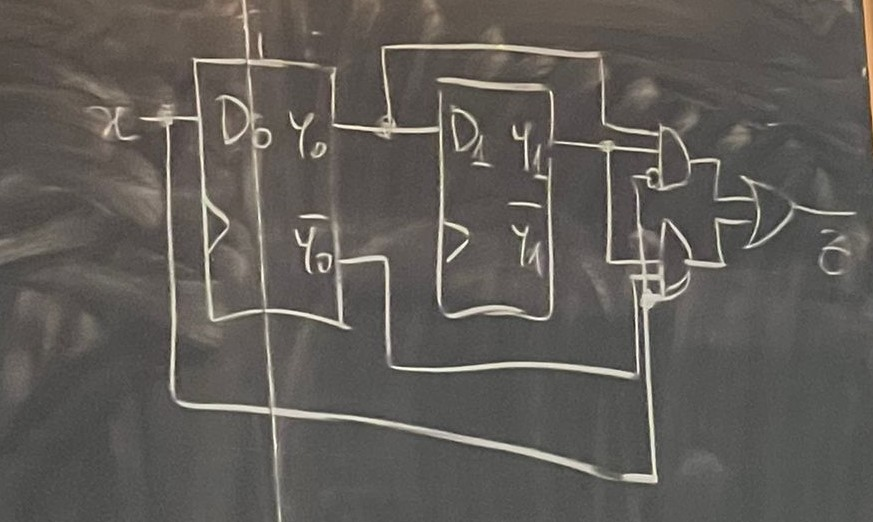
\includegraphics[width = 8cm]{images/es_retiseq1.jpeg}
    \caption{Rete sequenziale dell'Esercizio \ref{es:sintesi_retseq}}
\end{figure}
\end{exercise}

\newpage
\begin{exercise}\label{ex:autom_tiang}
    Ipotizziamo di avere la seguente tabella dell'automa:
    
    \begin{table}[ht]
    \centering
    \begin{tabular}{|c|c|c|}
         \hline& 0 & 1\\\hline
         A& \diagbox[width=1cm]{G}{00} & \diagbox[width=1cm]{C}{01}\\\hline
         B& \diagbox[width=1cm]{G}{00} & \diagbox[width=1cm]{D}{01}\\\hline
         C& \diagbox[width=1cm]{D}{10} & \diagbox[width=1cm]{A}{01}\\\hline
         D& \diagbox[width=1cm]{C}{10} & \diagbox[width=1cm]{B}{01}\\\hline
         E& \diagbox[width=1cm]{G}{00} &\diagbox[width=1cm]{F}{01}\\\hline
         F& \diagbox[width=1cm]{F}{10} & \diagbox[width=1cm]{E}{01}\\\hline
         G& \diagbox[width=1cm]{A}{01} &\diagbox[width=1cm]{F}{11}\\\hline
    \end{tabular}
\end{table}

Rappresentiamo in tabella triangolare gli stati e le eventuali equivalenze:

\begin{table}[ht]
    \centering
    \begin{tabular}{|c||*{7}{c|}}
                                   \cline{1-2}
      B & CD                 \\ \cline{1-3}
      C & X & X             \\ \cline{1-4}
      D & X & X & AB             \\ \cline{1-5}
      E & CF & DF & X & X         \\ \cline{1-6}
      F & X & X & DE,AE & CF,BE & X     \\ \cline{1-7}
      G & X & X & X & X & X & X \\ \hline\hline
      &A &B &C &D &E &F\\\hline
    \end{tabular}
\end{table}

Notiamo come, in questo caso, non trovando stati equivalenti nella tabella triangolare abbiamo bisogno di costruire un cosidetto grafo delle equivalenze che collega i punti degli stati che presentano delle equivalenze "numeriche".

\begin{figure}[H]
    \centering
    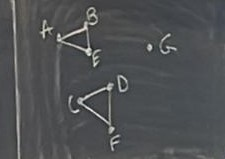
\includegraphics[width = 5cm]{images/grado_delle_equival.jpeg}
    \caption{Grafo delle equivalenze}
\end{figure}

Otteniamo così le forme:
\begin{equation*}
    Q_0=A'=\{A,B,E\}\hspace{0.5cm}Q_1=C'=\{C,D,F\}\hspace{0.5cm}Q_2=G
\end{equation*}

Riscriviamo la tabella dell'automa con il raggruppamento a stati appena svolto:
\begin{table}[ht]
    \centering
    \begin{tabular}{|c|c|c|}
         \hline& 0 & 1\\\hline
         $Q_0$& \diagbox[width=1cm]{$Q_2$}{00} & \diagbox[width=1cm]{$Q_1$}{01}\\\hline
         $Q_1$& \diagbox[width=1cm]{$Q_1$}{10} & \diagbox[width=1cm]{$Q_0$}{01}\\\hline
         $Q_2$& \diagbox[width=1cm]{$Q_0$}{01} & \diagbox[width=1cm]{$Q_1$}{11}\\\hline
    \end{tabular}
\end{table}

Gli stati e le uscite sono date, come sempre, dal valore che ci viene restituito se a $Q_0$ passiamo prima 0 e poi 1. Infatti $Q_0$ segue l'andamento di A,B,E che con input 0 ci portano a $G\backslash00$ quindi a $Q_2\backslash00$.

Rappresentiamo infine con gli automi di Mealy e Moore:
\begin{figure}[ht]
    \centering
    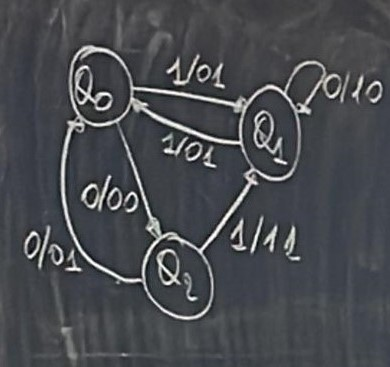
\includegraphics[height = 5cm]{images/es_mealy.jpeg}\hspace{0.5cm}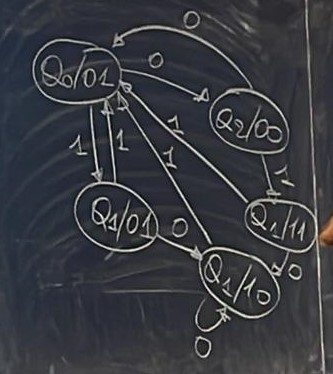
\includegraphics[height = 5cm]{images/es_moore.jpeg}
\end{figure}
\end{exercise}

\begin{exercise}\label{ex:minimizz_automa}
    Si minimizzi il seguente automa e si disegni l’automa minimo sia secondo il modello di Mealy che secondo il modello di Moore.
    \begin{figure}[H]
        \centering
        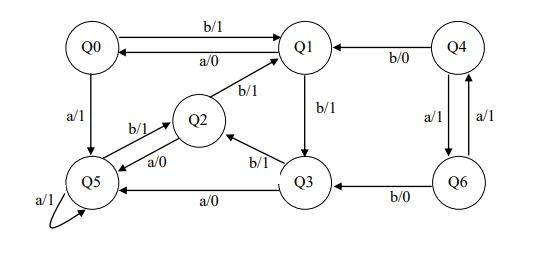
\includegraphics[width = 11cm]{images/es_minimizzautoma.JPG}
        \caption{Diagramma dell'automa}
    \end{figure}
    
    \begin{enumerate}
        \item Scrivo la tavola dell'automa:
        \begin{table}[H]
            \centering
            \begin{tabular}{|c|c|c|}
                 \hline& a & b\\\hline
                 $Q_0$& \diagbox[width=1cm]{$Q_5$}{1} & \diagbox[width=1cm]{$Q_1$}{1}\\\hline
                 $Q_1$& \diagbox[width=1cm]{$Q_0$}{0} & \diagbox[width=1cm]{$Q_3$}{1}\\\hline
                 $Q_2$& \diagbox[width=1cm]{$Q_5$}{1} & \diagbox[width=1cm]{$Q_1$}{1}\\\hline
                 $Q_3$& \diagbox[width=1cm]{$Q_5$}{0} & \diagbox[width=1cm]{$Q_2$}{1}\\\hline
                 $Q_4$& \diagbox[width=1cm]{$Q_6$}{1} & \diagbox[width=1cm]{$Q_1$}{0}\\\hline
                 $Q_5$& \diagbox[width=1cm]{$Q_5$}{1} & \diagbox[width=1cm]{$Q_2$}{1}\\\hline
                 $Q_6$& \diagbox[width=1cm]{$Q_4$}{1} & \diagbox[width=1cm]{$Q_3$}{0}\\\hline
            \end{tabular}
            \caption{Tavola dell'automa}
        \end{table}
        
        \item Minimizzo tramite la tabella triangolare:
        \begin{table}[H]
            \centering
            \begin{tabular}{|c||*{7}{c|}}
                                           \cline{1-2}
              $Q_1$ & X                 \\ \cline{1-3}
              $Q_2$ & X & 05,13             \\ \cline{1-4}
              $Q_3$ & X & 05,13 & 12             \\ \cline{1-5}
              $Q_4$ & x & X & X & X         \\ \cline{1-6}
              $Q_5$ & 12 & X & X & X & X     \\ \cline{1-7}
              $Q_6$ & X & X & X & X & 13 & X \\ \hline\hline
              &$Q_0$ &$Q_1$ &$Q_2$ &$Q_3$ &$Q_4$ &$Q_5$\\\hline
            \end{tabular}
            \caption{Tabella triangolare}
        \end{table}
        
        Scriviamo sottoforma di grafi gli stati equivalenti:
        \begin{figure}[ht]
            \centering
            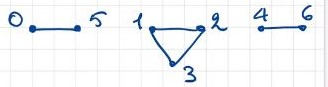
\includegraphics[width = 6cm]{images/grafi_es.JPG}
        \end{figure}
        \begin{equation*}
            Q'_0=\{Q_0,Q_5\}\hspace{1cm}Q'_1=\{Q_1,Q_2,Q_3\}\hspace{1cm}Q'_4=\{Q_4,Q_6\}
        \end{equation*}
        
        \item Rappresentiamo infine la tavola dell'automa minima. Guradando nella tabella di partenza gli stati mi chiedo: in che stato mi portano e che output producono?
        \begin{table}[ht]
        \centering
        \begin{tabular}{|c|c|c|}
                 \hline& a & b\\\hline
                 $Q'_0$& \diagbox[width=1cm]{$Q'_0$}{1} & \diagbox[width=1cm]{$Q'_1$}{1}\\\hline
                 $Q'_1$& \diagbox[width=1cm]{$Q'_0$}{0} & \diagbox[width=1cm]{$Q'_1$}{1}\\\hline
                 $Q'_4$& \diagbox[width=1cm]{$Q'_4$}{1} & \diagbox[width=1cm]{$Q'_1$}{1}\\\hline
            \end{tabular}
            \caption{Tavola minima dell'automa}
        \end{table}
        
        
    \end{enumerate}
\end{exercise}

\begin{exercise}
    Progettare la rete sequenziale che riceve in ingresso due sequenze di bit $x_1$ e $x_0$ e produce due uscite $z_1$ e $z_0$ che vengono poste ad 1 in accordo agli ultimi quattro bit ricevuti in ingresso nel modo seguente:
    \begin{itemize}
        \item se nessuno dei bit di ingresso è posto ad 1 oppure un solo bit di ingresso è posto ad 1, allora $z_1=z_0=0$;
        \item se due qualunque bit di ingresso sono posti ad 1, allora $z_1=0$ e $z_0=1$;
        \item se tre qualunque bit di ingresso sono posti ad 1, allora $z_1=1$ e $z_0=0$;
        \item se tutti e quattro gli ultimi bit ricevuti in ingresso sono posti ad 1, allora $z_1=1$ e $z_0=1$.
    \end{itemize}

La rete produce due ulteriori uscite A (allarme) e W (warning) tali che A è posta a 1 se le due uscite $z_1$ e $z_0$ sono 1, W è posta a 1 se una delle due uscite $z_1$ e $z_0$ è posta a 1 (ma non lo sono entrambe).
Si assuma che il primo valore in uscita prodotto per tutti i bit sia 0.

Si realizzi la rete usando un flip-flop di tipo T per il bit più significativo e di tipo JK per il meno significativo. 
Si realizzino le uscite $z_1$ e $z_0$ con ROM e le uscite A e W con porte logiche.

A questo punto possiamo procedere in due modi diversi. Ovvero possiamo assumere che la rete parta con la memoria azzerata (metodo più efficiente) o possiamo partire senza aver ricevuto alcun bit.

\begin{enumerate}
    \item Disegnamo la tabella dell'automa:
    
    $Q_0$ bit in memoria 00;
    
    $Q_1$ bit in memoria 01;
    
    $Q_2$ bit in memoria 10;
    
    $Q_3$ bit in memoria 11;
    
    \begin{table}[ht]
    \centering
    \begin{tabular}{|c|c|c|c|c|}
         \hline& $x_1x_0$ & $x_1x_0$ & $x_1x_0$ & $x_1x_0$\\
         & 00 & 01 & 10 & 11\\\hline
         $Q_0$& \diagbox[width=1cm]{$Q_0$}{00} & \diagbox[width=1cm]{$Q_1$}{00}& \diagbox[width=1cm]{$Q_2$}{00}& \diagbox[width=1cm]{$Q_3$}{01}\\\hline
         $Q_1$& \diagbox[width=1cm]{$Q_0$}{00} & \diagbox[width=1cm]{$Q_1$}{01}& \diagbox[width=1cm]{$Q_2$}{01}& \diagbox[width=1cm]{$Q_3$}{10}\\\hline
         $Q_2$& \diagbox[width=1cm]{$Q_0$}{00} & \diagbox[width=1cm]{$Q_1$}{01}& \diagbox[width=1cm]{$Q_2$}{01}& \diagbox[width=1cm]{$Q_3$}{10}\\\hline
         $Q_3$& \diagbox[width=1cm]{$Q_0$}{01} & \diagbox[width=1cm]{$Q_1$}{10}& \diagbox[width=1cm]{$Q_2$}{10}& \diagbox[width=1cm]{$Q_3$}{11}\\\hline
    \end{tabular}
    \caption{Tabella dell'automa}
    \end{table}

    Notiamo come gli stati $Q_1$ e $Q_2$ sono equivalenti possiamo pertanto scrivere: $Q'_1=\{Q_1,Q_2\}$
    
    \item Con le informazioni ottenute dalla tabella dell'automa possiamo reppresentarlo:
    \begin{figure}[ht]
        \centering
        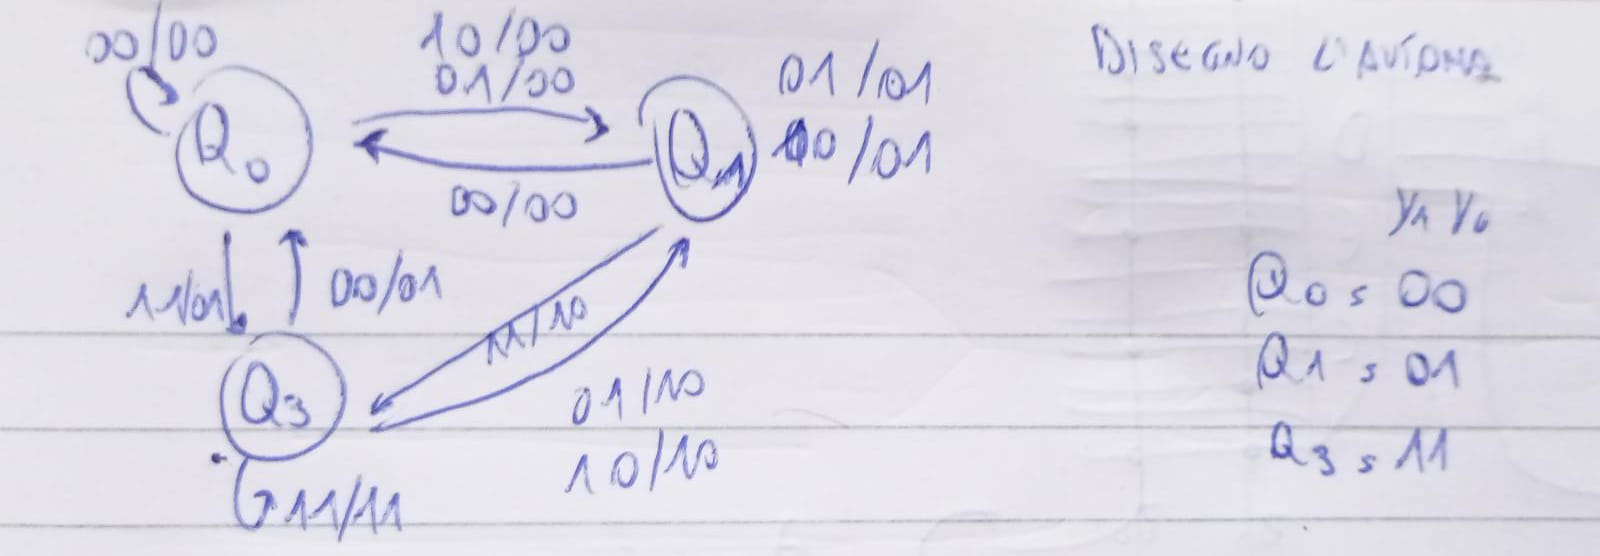
\includegraphics[width = 10cm]{images/diag_autom_escasa.jpeg}
        \caption{Diagramma dell'automa}
    \end{figure}
    
    \item Scriviamo ora la tavola degli stati futuri, guardando per gli ingressi $x_1$ e $x_0$ nella tabella dell'automa e riportando lo stato futuro e l'uscita. Per le funzioni di eccitazione, invece, guardo lo sato attuale e quello futuro e compilo i FF:
    
    \begin{table}[ht]
        \centering
        \begin{tabular}{|c|c|c|c|c|}
        \hline $x_1x_0y_1y_0$ & $Y_1Y_0$ & $z_1z_0$ & $T_1$ & $J_0K_0$\\\hline\hline
            0000 & 00 & 00 & 0 & 0-\\
            0001 & 00 & 00 & 0 & -1\\
            0010 & -- & -- & - & --\\
            0011 & 00 & 01 & 1 & -1\\\hline
            0100 & 01 & 00 & 0 & 1-\\
            0101 & 01 & 01 & 0 & -0\\
            0110 & -- & -- & - & --\\
            0111 & 01 & 10 & 1 & -0\\\hline
            1000 & 01 & 00 & 0 & 1-\\
            1001 & 01 & 01 & 0 & -0\\
            1010 & -- & -- & - & --\\
            1011 & 01 & 00 & 1 & -0\\\hline
            1100 & 11 & 01 & 1 & 1-\\
            1101 & 11 & 10 & 1 & -0\\
            1110 & -- & -- & - & --\\
            1111 & 11 & 11 & 0 & -0\\\hline
        \end{tabular}
        \caption{Tavola degli stati futuri}
    \end{table}
    
    \item Con le k-mappe trovaimo le espressioni minime delle funzioni di eccitazione:
    \begin{center}
    $T_1$ = 
    \begin{tabular}{|c|c|c|c|c|}
        \hline \diagbox[width=1.5cm]{$x_1x_0$}{$y_1y_0$} & 00 & 01 & 11 & 10 \\\hline\hline
        00 & 0 & 0 & 1 & -\\\hline
        01 & 0 & 0 & 1 & -\\\hline
        11 & 1 & 1 & 0 & -\\\hline
        10 & 0 & 0 & 1 & -\\\hline
    \end{tabular} = $\overline{x_1}y_1+\overline{x_0}y_1+x_1x_0\overline{y_1}$
    \end{center}
    \begin{center}
    $J_0$ = 
    \begin{tabular}{|c|c|c|c|c|}
        \hline \diagbox[width=1.5cm]{$x_1x_0$}{$y_1y_0$} & 00 & 01 & 11 & 10 \\\hline\hline
        00 & 0 & - & - & -\\\hline
        01 & 1 & - & - & -\\\hline
        11 & 1 & - & - & -\\\hline
        10 & 1 & - & - & -\\\hline
    \end{tabular} = $x_0+x_1$
    \end{center}
    \begin{center}
    $K_0$ = 
    \begin{tabular}{|c|c|c|c|c|}
        \hline \diagbox[width=1.5cm]{$x_1x_0$}{$y_1y_0$} & 00 & 01 & 11 & 10 \\\hline\hline
        00 & - & 1 & 1 & -\\\hline
        01 & - & 0 & 0 & -\\\hline
        11 & - & 0 & 0 & -\\\hline
        10 & - & 0 & 0 & -\\\hline
    \end{tabular} = $\overline{x_1}\overline{x_0}$
    \end{center}
    
    \item Possiamo ora disegnare il nostro circuito con le specifiche della traccia:
    \begin{figure}[ht]
        \centering
        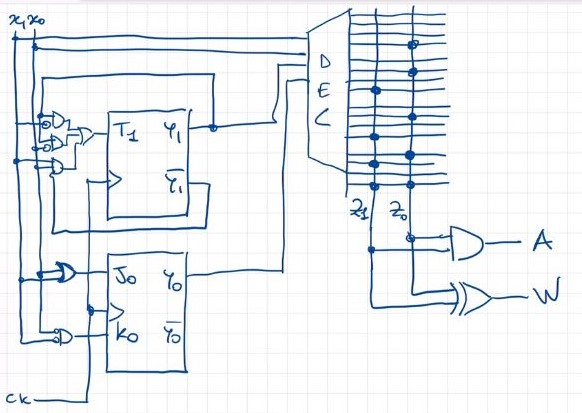
\includegraphics[width = 10cm]{images/es_circuito_casa.JPG}
        \caption{Circuito finale}
    \end{figure}
    
\end{enumerate}
\end{exercise}